\documentclass{exam}
\usepackage[paperwidth=210mm, paperheight=297mm, margin=2cm]{geometry}
\usepackage[utf8]{inputenc}
%\usepackage{ebgaramond-maths}

%==Math & Physics Packages==
\usepackage{amsmath, amsthm, amsfonts, amssymb}
\allowdisplaybreaks
\usepackage{setspace}
\usepackage{physics}
\usepackage{cancel}
\usepackage{nicefrac}

%==Image-related Packages==
\usepackage{graphics, graphicx}
\usepackage{tikz}
\usetikzlibrary{arrows.meta}
\usepackage{pgfplots}
\pgfplotsset{compat=1.18}
\usepackage{xcolor}
\usepackage{fourier-orns}

%==Colour Palette==
\definecolor{merah}{HTML}{F4564E}
\definecolor{merahtua}{HTML}{89313E}
\definecolor{biru}{HTML}{60BBE5}
\definecolor{birutua}{HTML}{412F66}
\definecolor{hijau}{HTML}{59CC78}
\definecolor{hijautua}{HTML}{366D5B}
\definecolor{kuning}{HTML}{FFD56B}
\definecolor{jingga}{HTML}{FBA15F}
\definecolor{ungu}{HTML}{8C5FBF}
\definecolor{lavender}{HTML}{CBA5E8}
\definecolor{merjamb}{HTML}{FFB6E0}

%==Theorems==
\usepackage{tcolorbox}
\tcbuselibrary{skins,breakable,theorems}
\usepackage{changepage}

\newcounter{hitung}
\setcounter{hitung}{\thesection}

\makeatletter
	% Solusi
	\def\tcb@theo@widetitle#1#2#3{\hbox to \textwidth{\textsc{\large#1}\normalsize\space#3\hfil(#2)}}
	\tcbset{
		theorem style/theorem wide name and number/.code={ \let\tcb@theo@title=\tcb@theo@widetitle},
		proofbox/.style={skin=enhancedmiddle,breakable,parbox=false,boxrule=0mm,
			check odd page, toggle left and right, colframe=black!20!white!92!hijau,
			leftrule=8pt, rightrule=0mm, boxsep=0mm,arc=0mm, outer arc=0mm,
			left=3mm,right=3mm,top=0mm,bottom=0mm, toptitle=0mm,
			bottomtitle=0mm,colback=gray!3!white!98!biru, before skip=8pt, after skip=8pt,
			before={\par\vskip-2pt},after={\par\smallbreak},
		},
	}
	\newtcolorbox{ProofBox}{proofbox}
	\makeatother
	
	\let\realproof\proof
	\let\realendproof\endproof
	\renewenvironment{proof}[1][Solusi.]{\ProofBox\strut\textsc{#1}\space}{\endProofBox}
        % Definition
	\newtcbtheorem[use counter=hitung, number within=section]{dfn}{Definisi}
	{theorem style=theorem wide name and number,breakable,enhanced,arc=0mm,outer arc=0mm,
		boxrule=0pt,toprule=1pt,leftrule=0pt,bottomrule=1pt, rightrule=0pt,left=0.2cm,right=0.2cm,
		titlerule=0.5em,toptitle=0.1cm,bottomtitle=-0.1cm,top=0.2cm,
		colframe=white!10!biru,colback=white!90!biru,coltitle=white,
            coltext=birutua!60!gray, title style={white!10!biru}, before skip=8pt, after skip=8pt,
		fonttitle=\bfseries,fontupper=\normalsize}{dfn}

	% Axiom
	\newtcbtheorem[use counter=hitung, number within=section]{axm}{Aksioma}
	{theorem style=theorem wide name and number,breakable,enhanced,arc=0mm,outer arc=0mm,
		boxrule=0pt,toprule=1pt,leftrule=0pt,bottomrule=1pt, rightrule=0pt,left=0.2cm,right=0.2cm,
		titlerule=0.5em,toptitle=0.1cm,bottomtitle=-0.1cm,top=0.2cm,
		colframe=white!10!biru,colback=white!90!biru,coltitle=white,
            coltext=birutua!60!gray, title style={white!10!biru}, before skip=8pt, after skip=8pt,
		fonttitle=\bfseries,fontupper=\normalsize}{axm}
 
	% Theorem
	\newtcbtheorem[use counter=hitung, number within=section]{thm}{Teorema}
	{theorem style=theorem wide name and number,breakable,enhanced,arc=0mm,outer arc=0mm,
		boxrule=0pt,toprule=1pt,leftrule=0pt,bottomrule=1pt, rightrule=0pt,left=0.2cm,right=0.2cm,
		titlerule=0.5em,toptitle=0.1cm,bottomtitle=-0.1cm,top=0.2cm,
		colframe=white!10!merah,colback=white!75!pink,coltitle=white, coltext=merahtua!80!merah,
		title style={white!10!merah}, before skip=8pt, after skip=8pt,
		fonttitle=\bfseries,fontupper=\normalsize}{thm}
	
	% Proposition
	\newtcbtheorem[use counter=hitung, number within=section]{prp}{Proposisi}
	{theorem style=theorem wide name and number,breakable,enhanced,arc=0mm,outer arc=0mm,
		boxrule=0pt,toprule=1pt,leftrule=0pt,bottomrule=1pt, rightrule=0pt,left=0.2cm,right=0.2cm,
		titlerule=0.5em,toptitle=0.1cm,bottomtitle=-0.1cm,top=0.2cm,
		colframe=white!10!hijau,colback=white!90!hijau,coltitle=white, coltext=hijautua!80!brown,
		title style={white!10!hijau}, before skip=8pt, after skip=8pt,
		fonttitle=\bfseries,fontupper=\normalsize}{prp}


	% Example
	\newtcolorbox[use counter=hitung, number within=section]{cth}[1][]{breakable,
		colframe=white!10!jingga, coltitle=white!90!jingga, colback=white!85!jingga, coltext=black!10!brown!50!jingga, colbacktitle=white!10!jingga, enhanced, fonttitle=\bfseries,fontupper=\normalsize, attach boxed title to top left={yshift=-2mm}, before skip=8pt, after skip=8pt,
		title=Contoh~\thetcbcounter \ \ #1}

	% Catatan/Note
	\newtcolorbox{ctt}[1][]{enhanced, 
		left=4.1mm, borderline west={8pt}{0pt}{white!10!kuning}, 
		before skip=6pt, after skip=6pt, 
		colback=white!85!kuning, colframe= white!85!kuning, coltitle=orange!60!kuning!25!brown, coltext=orange!60!kuning!25!brown,
		fonttitle=\bfseries,fontupper=\normalsize, before skip=8pt, after skip=8pt,
		title=\underline{Catatan}  #1}
	
	% Komentar/Remark
	\newtcolorbox{rmr}[1][]{%
		,arc=0mm,outer arc=0mm,
		boxrule=0pt,toprule=1pt,leftrule=0pt,bottomrule=5pt, rightrule=0pt,left=0.2cm,right=0.2cm,
		titlerule=0.5em,toptitle=0.1cm,bottomtitle=-0.1cm,top=0.2cm,
		colframe=white!10!kuning,colback=white!85!kuning,coltitle=white, coltext=orange!60!kuning,
		fonttitle=\bfseries,fontupper=\normalsize, before skip=8pt, after skip=8pt,
		title=Komentar  #1}

\usepackage{xpatch}

\makeatletter
\xpatchcmd{\@fillin@relay}
  {\hbox to #1{\hrulefill}\fi}
  {\hbox{\framebox[#1]{\rule{0pt}{2ex}}}\fi}
  {}{}
\makeatother

%==Formatting Packages==
\usepackage{multicol}
\usepackage{multirow}
\usepackage{enumitem}
\usepackage{indentfirst}
%==Layouting Packages==
\usepackage{titlesec}
\footer{}{\thepage}{}  
\newcommand{\fpb}[2]{\mathrm{FPB}(#1, #2)}
\newcommand{\kpk}[2]{\mathrm{KPK}(#1, #2)}
 
%Reference and Bibliography Packages==
\usepackage{hyperref}
\hypersetup{
    colorlinks=true,
    linkcolor={black},
    citecolor={biru!70!black},
    urlcolor={biru!80!black}
}

\numberwithin{equation}{section}

\renewcommand{\mod}{\mathrm{mod} \ }


%Titling
\newcommand{\garis} [3] []{
	\begin{center}
		\begin{tikzpicture}
			\draw[#2-#3, ultra thick, #1] (0,0) to (1\linewidth,0);
		\end{tikzpicture}
	\end{center}
}

\title{\vspace{-2em}Solusi Ujian Reevaluasi MA1101 2022}
\author{BPA Akademik STEI-K 2023}
\date{20 Desember 2023}

\begin{document}
\maketitle
\vspace{-3em}
\garis{Kite}{Kite}

\section*{Bagian A}
\begin{enumerate}
    \item 
    \begin{enumerate}
        \item Himpunan penyelesaian pertidaksamaan $x^2 - 9 > 0$ adalah $\fillin$
        \item Daerah asal fungsi $f(x) = \sqrt{9 - x^2}$ adalah $D_f = \fillin$
    \end{enumerate}
    \begin{proof}
        \begin{enumerate}[label=(\alph*)]
            \item $x^2 - 9 > 0 \iff {\color{red}(x + 3)}{\color{blue}(x - 3)} > 0$. Selanjutnya, cek tanda $\pm$-nya pada garis bilangan:
            {\centering
            

\tikzset{every picture/.style={line width=0.75pt}} %set default line width to 0.75pt        

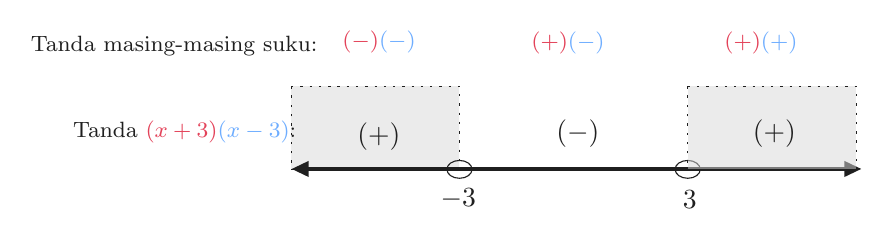
\begin{tikzpicture}[x=0.75pt,y=0.75pt,yscale=-1,xscale=1]
%uncomment if require: \path (0,124); %set diagram left start at 0, and has height of 124

%Shape: Rectangle [id:dp46283291881464317] 
\draw  [color={rgb, 255:red, 31; green, 31; blue, 31 }  ,draw opacity=1 ][fill={rgb, 255:red, 215; green, 215; blue, 215 }  ,fill opacity=0.5 ][dash pattern={on 0.84pt off 2.51pt}] (130.92,57.2) -- (212.04,57.2) -- (212.04,97.2) -- (130.92,97.2) -- cycle ;
%Straight Lines [id:da5592558548969113] 
\draw [color={rgb, 255:red, 31; green, 31; blue, 31 }  ,draw opacity=1 ][line width=1.5]    (135.27,97) -- (401.6,97) ;
\draw [shift={(405.6,97)}, rotate = 180] [fill={rgb, 255:red, 31; green, 31; blue, 31 }  ,fill opacity=1 ][line width=0.08]  [draw opacity=0] (8.13,-3.9) -- (0,0) -- (8.13,3.9) -- cycle    ;
\draw [shift={(131.27,97)}, rotate = 0] [fill={rgb, 255:red, 31; green, 31; blue, 31 }  ,fill opacity=1 ][line width=0.08]  [draw opacity=0] (8.13,-3.9) -- (0,0) -- (8.13,3.9) -- cycle    ;
%Shape: Ellipse [id:dp47417300949069885] 
\draw  [color={rgb, 255:red, 31; green, 31; blue, 31 }  ,draw opacity=1 ] (205.99,97.2) .. controls (205.99,94.83) and (208.7,92.9) .. (212.04,92.9) .. controls (215.39,92.9) and (218.1,94.83) .. (218.1,97.2) .. controls (218.1,99.57) and (215.39,101.5) .. (212.04,101.5) .. controls (208.7,101.5) and (205.99,99.57) .. (205.99,97.2) -- cycle ;
%Shape: Ellipse [id:dp6444087413829098] 
\draw  [color={rgb, 255:red, 31; green, 31; blue, 31 }  ,draw opacity=1 ] (315.95,97.2) .. controls (315.95,94.83) and (318.66,92.9) .. (322.01,92.9) .. controls (325.35,92.9) and (328.06,94.83) .. (328.06,97.2) .. controls (328.06,99.57) and (325.35,101.5) .. (322.01,101.5) .. controls (318.66,101.5) and (315.95,99.57) .. (315.95,97.2) -- cycle ;
%Shape: Rectangle [id:dp35146469083956533] 
\draw  [color={rgb, 255:red, 31; green, 31; blue, 31 }  ,draw opacity=1 ][fill={rgb, 255:red, 215; green, 215; blue, 215 }  ,fill opacity=0.5 ][dash pattern={on 0.84pt off 2.51pt}] (322.01,57.2) -- (403.13,57.2) -- (403.13,97.2) -- (322.01,97.2) -- cycle ;

% Text Node
\draw (201.65,105.2) node [anchor=north west][inner sep=0.75pt]  [color={rgb, 255:red, 31; green, 31; blue, 31 }  ,opacity=1 ]  {$-3$};
% Text Node
\draw (318.42,106.2) node [anchor=north west][inner sep=0.75pt]  [color={rgb, 255:red, 31; green, 31; blue, 31 }  ,opacity=1 ]  {$3$};
% Text Node
\draw (161.59,73.56) node [anchor=north west][inner sep=0.75pt]  [color={rgb, 255:red, 31; green, 31; blue, 31 }  ,opacity=1 ]  {$( +)$};
% Text Node
\draw (257.44,72.2) node [anchor=north west][inner sep=0.75pt]  [color={rgb, 255:red, 31; green, 31; blue, 31 }  ,opacity=1 ]  {$( -)$};
% Text Node
\draw (352.09,72.2) node [anchor=north west][inner sep=0.75pt]  [color={rgb, 255:red, 31; green, 31; blue, 31 }  ,opacity=1 ]  {$( +)$};
% Text Node
\draw (154.41,29.2) node [anchor=north west][inner sep=0.75pt]  [font=\footnotesize,color={rgb, 255:red, 227; green, 67; blue, 89 }  ,opacity=1 ]  {$\textcolor[rgb]{0.89,0.26,0.35}{( -)}\textcolor[rgb]{0.43,0.68,1}{( -)}$};
% Text Node
\draw (4.27,31.73) node [anchor=north west][inner sep=0.75pt]  [font=\footnotesize,color={rgb, 255:red, 31; green, 31; blue, 31 }  ,opacity=1 ] [align=left] {Tanda masing-masing suku:};
% Text Node
\draw (24.6,72.6) node [anchor=north west][inner sep=0.75pt]  [font=\footnotesize,color={rgb, 255:red, 31; green, 31; blue, 31 }  ,opacity=1 ] [align=left] {Tanda $\displaystyle \textcolor[rgb]{0.89,0.26,0.35}{( x+3)}\textcolor[rgb]{0.43,0.68,1}{( x-3)}$:};
% Text Node
\draw (245.41,29.86) node [anchor=north west][inner sep=0.75pt]  [font=\footnotesize]  {$\textcolor[rgb]{0.89,0.26,0.35}{( +)}\textcolor[rgb]{0.43,0.68,1}{( -)}$};
% Text Node
\draw (338.41,29.86) node [anchor=north west][inner sep=0.75pt]  [font=\footnotesize]  {$\textcolor[rgb]{0.89,0.26,0.35}{( +)}\textcolor[rgb]{0.43,0.68,1}{( +)}$};


\end{tikzpicture}

            \par}
            Jadi, himpunan penyelesaian pertidaksamaan tersebut adalah $(-\infty, -3) \cup (3, \infty)$. \qed
            \item Fungsi akar kuadrat akan menjadi tak terdefinisi jika ekspresi di dalamnya bernilai negatif. Jadi, ekspresi di dalam akar harus lebih besar atau sama dengan nol:
            \[9 - x^2 > 0 \iff x^2 - 9 < 0\]
            Dari cek tanda yang dilakukan pada bagian (a), nampak bahwa pertidaksamaan di atas berlaku pada selang $(-3, 3)$. Dengan demikian, $D_f = (-3, 3)$. \qed
        \end{enumerate}
    \end{proof}\vspace{1em}
    \item Diberikan grafik fungsi $f$ sebagai berikut.
    
    {\centering
        \tikzset{every picture/.style={line width=0.75pt}} %set default line width to 0.75pt        
        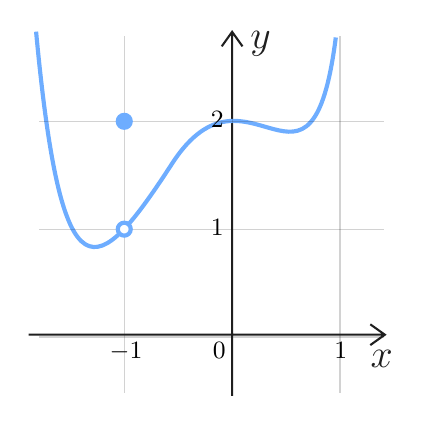
\begin{tikzpicture}[x=0.75pt,y=0.75pt,yscale=-1,xscale=1]
            %uncomment if require: \path (0,180); %set diagram left start at 0, and has height of 180
            
            %Shape: Axis 2D [id:dp46384820360546564] 
            \draw [color={rgb, 255:red, 31; green, 31; blue, 31 }  ,draw opacity=1 ][line width=0.75]  (1.53,148.66) -- (173.11,148.66) (99.53,2.74) --         (99.53,178.18) (166.11,143.66) -- (173.11,148.66) -- (166.11,153.66) (94.53,9.74) -- (99.53,2.74) --     (104.53,9.74)  ;
            %Curve Lines [id:da03444933884197443] 
            \draw [color={rgb, 255:red, 110; green, 173; blue, 255 }  ,draw opacity=1 ][line width=1.5]    (5.08,2.65) .. controls  (17.48,134.5) and       (33.88,122.74) .. (70.68,66.1) .. controls (107.48,9.45) and (137.48,98.9) .. (149.48,5.45) ;
            %Shape: Grid [id:dp1775755329667379] 
            \draw  [draw opacity=0] (6.56,4.84) -- (172.76,4.84) -- (172.76,176.57) -- (6.56,176.57) -- cycle ; \draw  [color={rgb, 255:red, 31; green, 31;         blue, 31 }  ,draw opacity=0.2 ] (47.56,4.84) -- (47.56,176.57)(99.53,4.84) -- (99.53,176.57)(151.5,4.84) --     (151.5,176.57) ; \draw  [color=     {rgb, 255:red, 31; green, 31; blue, 31 }  ,draw opacity=0.2 ] (6.56,45.84) -- (172.76,45.84)(6.56,97.81) -- (172.76,97.81)(6.56,149.78) --      (172.76,149.78) ; \draw  [color={rgb, 255:red, 31; green, 31; blue, 31 }  ,draw   opacity=0.2 ]  ;
            %Shape: Circle [id:dp41952777311759415] 
            \draw  [color={rgb, 255:red, 110; green, 173; blue, 255 }  ,draw opacity=1 ][fill={rgb, 255:red, 110; green, 173; blue, 255 }   ,fill opacity=1 ]       [line width=1.5]  (44.44,45.84) .. controls (44.44,44.12) and (45.84,42.72) .. (47.56,42.72) .. controls (49.28,42.72) and (50.68,44.12) ..     (50.68,45.84) .. controls (50.68,47.57) and (49.28,48.96) .. (47.56,48.96) .. controls  (45.84,48.96) and (44.44,47.57) .. (44.44,45.84) -- cycle    ;
            %Shape: Circle [id:dp3582801459779028] 
            \draw  [color={rgb, 255:red, 110; green, 173; blue, 255 }  ,draw opacity=1 ][fill={rgb, 255:red, 255; green, 255; blue, 255 }   ,fill opacity=1 ]       [line width=1.5]  (44.44,97.81) .. controls (44.44,96.09) and (45.84,94.69) .. (47.56,94.69) .. controls (49.28,94.69) and (50.68,96.09) ..     (50.68,97.81) .. controls (50.68,99.54) and (49.28,100.93) .. (47.56,100.93) .. controls    (45.84,100.93) and (44.44,99.54) .. (44.44,97.81) --     cycle ;
            
            % Text Node
            \draw (107,1) node [anchor=north west][inner sep=0.75pt]  [font=\Large,color={rgb, 255:red, 31; green, 31; blue, 31 }    ,opacity=1 ]        {$y$};
            % Text Node
            \draw (165,155) node [anchor=north west][inner sep=0.75pt]  [font=\Large,color={rgb, 255:red, 31; green, 31; blue, 31 }    ,opacity=1 ]        {$x$};
            % Text Node
            \draw (88,91.7) node [anchor=north west][inner sep=0.75pt]  [font=\small] [align=left] {$\displaystyle 1$};
            % Text Node
            \draw (88,39.7) node [anchor=north west][inner sep=0.75pt]  [font=\small] [align=left] {2};
            % Text Node
            \draw (147.5,151) node [anchor=north west][inner sep=0.75pt]  [font=\small] [align=left] {$\displaystyle 1$};
            % Text Node
            \draw (39.23,151) node [anchor=north west][inner sep=0.75pt]  [font=\small] [align=left] {$\displaystyle -1$};
            % Text Node
            \draw (89,151) node [anchor=north west][inner sep=0.75pt]  [font=\small] [align=left] {$\displaystyle 0$};
        \end{tikzpicture}
    \par}
    \begin{enumerate}
        \item $f(-1) = \fillin$
        \item $\displaystyle \lim_{x \to -1} f(x) = \fillin$
    \end{enumerate}
    \begin{proof}
        \begin{enumerate}[label=(\alph*)]
            \item $f(-1) = 2$ karena titik tertutup ada di $(-1, 2)$. \\ 
            NB: Titik berlubang pada $(-1, 1)$ menandakan bahwa $f(-1) \neq 1$. 
            \item Nampak bahwa nilai $f$ mendekati $1$ ketika $x$ mendekati $-1$ baik dari sisi kiri maupun sisi kanan, yakni
            \[\lim_{x \to -1^-} f(x) = \lim_{x \to -1^+} f(x) = 1\]
            sehingga $\displaystyle \lim_{x \to -1} f(x) = 1$. \qed
        \end{enumerate}
    \end{proof}\vspace{1em}
    
    \item Grafik fungsi $f$ dan daerah $R_1$ dan $R_2$ diberikan sebagai berikut.
    
    {\centering
        

\tikzset{every picture/.style={line width=0.75pt}} %set default line width to 0.75pt        

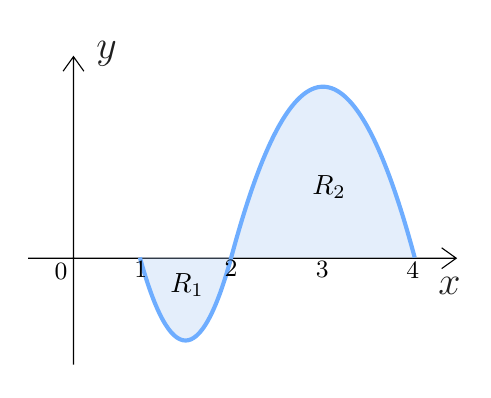
\begin{tikzpicture}[x=0.75pt,y=0.75pt,yscale=-1,xscale=1]
%uncomment if require: \path (0,158); %set diagram left start at 0, and has height of 158

%Shape: Axis 2D [id:dp26400090933574605] 
\draw  (-6.4,106.94) -- (199.8,106.94)(15.4,9.83) -- (15.4,158.26) (192.8,101.94) -- (199.8,106.94) -- (192.8,111.94) (10.4,16.83) -- (15.4,9.83) -- (20.4,16.83)  ;
%Shape: Parabola [id:dp7388591996543863] 
\draw  [color={rgb, 255:red, 110; green, 173; blue, 255 }  ,draw opacity=1 ][fill={rgb, 255:red, 164; green, 198; blue, 243 }  ,fill opacity=0.3 ][line width=1.5]  (47.4,106.6) .. controls (62.07,159.93) and (76.73,159.93) .. (91.4,106.6) ;
%Shape: Parabola [id:dp041425754385784774] 
\draw  [color={rgb, 255:red, 110; green, 173; blue, 255 }  ,draw opacity=1 ][fill={rgb, 255:red, 164; green, 198; blue, 243 }  ,fill opacity=0.3 ][line width=1.5]  (91.4,106.6) .. controls (120.87,-3.13) and (150.33,-3.13) .. (179.8,106.6) ;

% Text Node
\draw (25.19,1.33) node [anchor=north west][inner sep=0.75pt]  [font=\Large,color={rgb, 255:red, 31; green, 31; blue, 31 }  ,opacity=1 ]  {$y$};
% Text Node
\draw (190,115) node [anchor=north west][inner sep=0.75pt]  [font=\Large,color={rgb, 255:red, 31; green, 31; blue, 31 }  ,opacity=1 ]  {$x$};
% Text Node
\draw (43.5,107) node [anchor=north west][inner sep=0.75pt]  [font=\small] [align=left] {$\displaystyle 1$};
% Text Node
\draw (5,108.4) node [anchor=north west][inner sep=0.75pt]  [font=\small] [align=left] {$\displaystyle 0$};
% Text Node
\draw (86.9,106.8) node [anchor=north west][inner sep=0.75pt]  [font=\small] [align=left] {$\displaystyle 2$};
% Text Node
\draw (130.9,107.4) node [anchor=north west][inner sep=0.75pt]  [font=\small] [align=left] {$\displaystyle 3$};
% Text Node
\draw (174.5,107.6) node [anchor=north west][inner sep=0.75pt]  [font=\small] [align=left] {$\displaystyle 4$};
% Text Node
\draw (60.8,113) node [anchor=north west][inner sep=0.75pt]    {$R_{1}$};
% Text Node
\draw (129.2,65.77) node [anchor=north west][inner sep=0.75pt]    {$R_{2}$};


\end{tikzpicture}
    \par}
    Jika luas daerah $R_1$ dan $R_2$ berturut-turut adalah $1$ satuan luas dan $6$ satuan luas maka
    \begin{enumerate}
        \item $\displaystyle \int_{4}^{2} f(x) \dd{x} =  \fillin$
        \item $\displaystyle \int_{1}^{4} f(x) \dd{x} =  \fillin$
    \end{enumerate}

    \begin{proof}
        Integral tentu dari suatu fungsi merepresentasikan luas bertanda dari daerah yang berada di bawah grafik fungsi tersebut. Luasan di bawah sumbu-$x$ ($y$-nya negatif) bernilai negatif, sedangkan luasan di atas sumbu-$x$ bernilai positif. Jadi, $-\displaystyle \int_{1}^{2} f(x) \dd{x}$ dan $\displaystyle \int_{2}^{4} f(x) \dd{x}$ secara berturut-turut sama dengan luas dari $R_1$ dan $R_2$.
        \begin{enumerate}[label=(\alph*)]
            \item Berdasarkan sifat integral untuk batas bawah yang lebih besar dari batas atas integrasi, kita dapatkan $\displaystyle \int_{4}^{2} f(x) \dd{x} = -\int_{2}^{4} f(x) \dd{x} = -6$. \qed
            \item Berdasarkan sifat aditif untuk integral, kita dapatkan $\displaystyle \int_{1}^{4} f(x) \dd{x} = \int_{1}^{2} f(x) \dd{x} + \int_{2}^{4} f(x) \dd{x} = -1 + 6 = 5$. \qed
        \end{enumerate}
    \end{proof}\vspace{1em}
    
\item Dengan substitusi $u = 2x + 7$, diperoleh
\[\int_{0}^{1} \sqrt{2x + 7} \dd{x} = \int_{7}^{b} g(u) \dd{u}\]
dengan
\begin{enumerate}
    \item $b = \fillin $
    \item $g(u) = \fillin$
\end{enumerate}

\begin{proof}
        Jika $u = 2x + 7$ maka menurunkan kedua ruas menghasilkan $\dd{u} = 2 \dd{x}$, atau $\dd{x} = \dfrac{\dd{u}}{2}$. 
        
        \par Selanjutnya, batas-batas integralnya perlu diganti menurut variabel $u$. Ketika $x = 0$, $u = 2(0) + 7 = 7$ dan ketika $x = 1$, $u = 2(1) + 7 = 9$. Jadi, batas bawah dan batas atasnya secara berturut-turut adalah $u = 7$ dan $u = 9$. 
        
        
        \par Dengan demikian, integral semula dapat ditulis kembali sebagai
        \[\int_{0}^{1} \sqrt{2x + 7} \dd{x} = \int_{7}^{9} \sqrt{u} \; \frac{\dd{u}}{2} = \int_{7}^{9} \frac{\sqrt{u}}{2} \dd{u}\]
        Mencocokkan dengan bentuk $\displaystyle \int_{7}^{b} g(u) \dd{u}$, kita dapatkan $b = 9$ dan $g(u) = \sqrt{u}/2$. \qed
    \end{proof}\vspace{1em}

\item Suatu daerah $R$ dibatasi oleh kurva $y = x^2$ dan garis $y = 9$, seperti diberikan pada gambar di bawah.

    {\centering 
\tikzset{every picture/.style={line width=0.75pt}} %set default line width to 0.75pt        

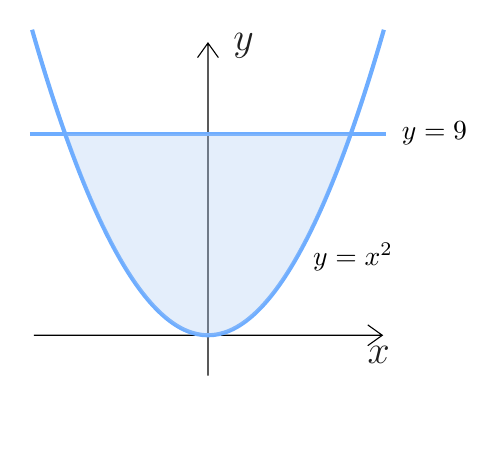
\begin{tikzpicture}[x=0.75pt,y=0.75pt,yscale=-1,xscale=1]
%uncomment if require: \path (0,188); %set diagram left start at 0, and has height of 188

%Shape: Axis 2D [id:dp26391451899144514] 
\draw  (26,158.98) -- (193.89,158.98)(109.89,18.18) -- (109.89,178.4) (186.89,153.98) -- (193.89,158.98) -- (186.89,163.98) (104.89,25.18) -- (109.89,18.18) -- (114.89,25.18)  ;
%Shape: Parabola [id:dp28908553763765954] 
\draw  [color={rgb, 255:red, 110; green, 173; blue, 255 }  ,draw opacity=1 ][line width=1.5]  (25.14,11.78) .. controls (81.64,208.05) and (138.14,208.05) .. (194.64,11.78) ;
%Straight Lines [id:da12505482028457338] 
\draw [color={rgb, 255:red, 110; green, 173; blue, 255 }  ,draw opacity=1 ][line width=1.5]    (24.03,61.98) -- (195.74,61.98) ;
%Shape: Parabola [id:dp13251624136445384] 
\draw  [draw opacity=0][fill={rgb, 255:red, 164; green, 198; blue, 243 }  ,fill opacity=0.3 ][line width=1.5]  (41.95,61.98) .. controls (87.24,191.31) and (132.53,191.31) .. (177.83,61.98) ;

% Text Node
\draw (120.84,12.28) node [anchor=north west][inner sep=0.75pt]  [font=\Large,color={rgb, 255:red, 31; green, 31; blue, 31 }  ,opacity=1 ]  {$y$};
% Text Node
\draw (185.54,163.15) node [anchor=north west][inner sep=0.75pt]  [font=\Large,color={rgb, 255:red, 31; green, 31; blue, 31 }  ,opacity=1 ]  {$x$};
% Text Node
\draw (202,55) node [anchor=north west][inner sep=0.75pt]    {$y=9$};
% Text Node
\draw (159.31,113.4) node [anchor=north west][inner sep=0.75pt]    {$y=x^{2}$};


\end{tikzpicture}
    \par}

Luas daerah $R$ adalah $\displaystyle\int_{-a}^{a} h(x) \dd{x}$ dengan
\begin{enumerate}
    \item $a = \fillin$
    \item $h(x) = \fillin$
\end{enumerate}

\begin{proof}
    Titik potong antara $y = x^2$ dan $y = 9$ adalah
    \begin{align*}
        x^2             &= 9 \\[.5em]
        x^2 - 9         &= 0 \\[.5em]
        (x - 3)(x + 3)  &= 0 \\[.5em]
        x = -3 &\lor x = 3
    \end{align*}    
    Didapatkan titik potong $x = -3$ dan $x = 3$. Perhatikan ilustrasi berikut.

    {\centering
    

\tikzset{every picture/.style={line width=0.75pt}} %set default line width to 0.75pt        

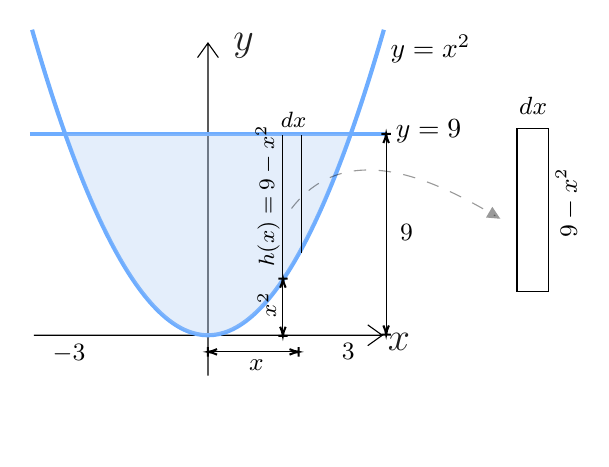
\begin{tikzpicture}[x=0.75pt,y=0.75pt,yscale=-1,xscale=1]
%uncomment if require: \path (0,188); %set diagram left start at 0, and has height of 188

%Shape: Axis 2D [id:dp6315151716853449] 
\draw  (26,158.98) -- (193.89,158.98)(109.89,18.18) -- (109.89,178.4) (186.89,153.98) -- (193.89,158.98) -- (186.89,163.98) (104.89,25.18) -- (109.89,18.18) -- (114.89,25.18)  ;
%Shape: Parabola [id:dp37763148866547547] 
\draw  [color={rgb, 255:red, 110; green, 173; blue, 255 }  ,draw opacity=1 ][line width=1.5]  (25.14,11.78) .. controls (81.64,208.05) and (138.14,208.05) .. (194.64,11.78) ;
%Straight Lines [id:da27377897829966646] 
\draw [color={rgb, 255:red, 110; green, 173; blue, 255 }  ,draw opacity=1 ][line width=1.5]    (24.03,61.98) -- (195.74,61.98) ;
%Shape: Parabola [id:dp3100100056741979] 
\draw  [draw opacity=0][fill={rgb, 255:red, 164; green, 198; blue, 243 }  ,fill opacity=0.3 ][line width=1.5]  (41.95,61.98) .. controls (87.24,191.31) and (132.53,191.31) .. (177.83,61.98) ;
%Straight Lines [id:da9354037621296771] 
\draw    (146,62.61) -- (146,131.65) ;
%Straight Lines [id:da5305819628055637] 
\draw    (155.08,62.61) -- (155.08,119.25) ;
%Straight Lines [id:da27204468673386106] 
\draw    (153.56,166.98) -- (109.89,166.98) ;
\draw [shift={(109.89,166.98)}, rotate = 360] [color={rgb, 255:red, 0; green, 0; blue, 0 }  ][line width=0.75]    (0,2.24) -- (0,-2.24)(4.37,-1.32) .. controls (2.78,-0.56) and (1.32,-0.12) .. (0,0) .. controls (1.32,0.12) and (2.78,0.56) .. (4.37,1.32)   ;
\draw [shift={(153.56,166.98)}, rotate = 180] [color={rgb, 255:red, 0; green, 0; blue, 0 }  ][line width=0.75]    (0,2.24) -- (0,-2.24)(4.37,-1.32) .. controls (2.78,-0.56) and (1.32,-0.12) .. (0,0) .. controls (1.32,0.12) and (2.78,0.56) .. (4.37,1.32)   ;
%Straight Lines [id:da0026194942798738463] 
\draw    (195.74,158.63) -- (195.74,61.98) ;
\draw [shift={(195.74,61.98)}, rotate = 90] [color={rgb, 255:red, 0; green, 0; blue, 0 }  ][line width=0.75]    (0,2.24) -- (0,-2.24)(4.37,-1.32) .. controls (2.78,-0.56) and (1.32,-0.12) .. (0,0) .. controls (1.32,0.12) and (2.78,0.56) .. (4.37,1.32)   ;
\draw [shift={(195.74,158.63)}, rotate = 270] [color={rgb, 255:red, 0; green, 0; blue, 0 }  ][line width=0.75]    (0,2.24) -- (0,-2.24)(4.37,-1.32) .. controls (2.78,-0.56) and (1.32,-0.12) .. (0,0) .. controls (1.32,0.12) and (2.78,0.56) .. (4.37,1.32)   ;
%Straight Lines [id:da8730274834118144] 
\draw    (146,159.25) -- (146,131.65) ;
\draw [shift={(146,131.65)}, rotate = 90] [color={rgb, 255:red, 0; green, 0; blue, 0 }  ][line width=0.75]    (0,2.24) -- (0,-2.24)(4.37,-1.32) .. controls (2.78,-0.56) and (1.32,-0.12) .. (0,0) .. controls (1.32,0.12) and (2.78,0.56) .. (4.37,1.32)   ;
\draw [shift={(146,159.25)}, rotate = 270] [color={rgb, 255:red, 0; green, 0; blue, 0 }  ][line width=0.75]    (0,2.24) -- (0,-2.24)(4.37,-1.32) .. controls (2.78,-0.56) and (1.32,-0.12) .. (0,0) .. controls (1.32,0.12) and (2.78,0.56) .. (4.37,1.32)   ;
%Curve Lines [id:da4398813049026853] 
\draw [color={rgb, 255:red, 0; green, 0; blue, 0 }  ,draw opacity=0.4 ] [dash pattern={on 4.5pt off 4.5pt}]  (150.14,97.9) .. controls (177.26,62.55) and (221.6,85.76) .. (248.33,101.43) ;
\draw [shift={(250.76,102.85)}, rotate = 210.58] [fill={rgb, 255:red, 0; green, 0; blue, 0 }  ,fill opacity=0.4 ][line width=0.08]  [draw opacity=0] (6.25,-3) -- (0,0) -- (6.25,3) -- cycle    ;
%Shape: Rectangle [id:dp9694480087804784] 
\draw   (258.8,59.2) -- (273.96,59.2) -- (273.96,138.05) -- (258.8,138.05) -- cycle ;

% Text Node
\draw (120.84,12.28) node [anchor=north west][inner sep=0.75pt]  [font=\Large,color={rgb, 255:red, 31; green, 31; blue, 31 }  ,opacity=1 ]  {$y$};
% Text Node
\draw (195.34,156.63) node [anchor=north west][inner sep=0.75pt]  [font=\Large,color={rgb, 255:red, 31; green, 31; blue, 31 }  ,opacity=1 ]  {$x$};
% Text Node
\draw (199.2,53.8) node [anchor=north west][inner sep=0.75pt]    {$y=9$};
% Text Node
\draw (196.64,12.98) node [anchor=north west][inner sep=0.75pt]    {$y=x^{2}$};
% Text Node
\draw (131.6,127.15) node [anchor=north west][inner sep=0.75pt]  [font=\footnotesize,rotate=-270]  {$h( x) =9-x^{2}$};
% Text Node
\draw (143.8,50.05) node [anchor=north west][inner sep=0.75pt]  [font=\footnotesize]  {$dx$};
% Text Node
\draw (128.4,169.55) node [anchor=north west][inner sep=0.75pt]  [font=\small]  {$x$};
% Text Node
\draw (201.2,104.4) node [anchor=north west][inner sep=0.75pt]  [font=\small]  {$9$};
% Text Node
\draw (132.6,151.49) node [anchor=north west][inner sep=0.75pt]  [font=\footnotesize,rotate=-270]  {$x^{2}$};
% Text Node
\draw (258.6,43.25) node [anchor=north west][inner sep=0.75pt]  [font=\small]  {$dx$};
% Text Node
\draw (276.1,113.3) node [anchor=north west][inner sep=0.75pt]  [font=\small,rotate=-270]  {$9-x^{2}$};
% Text Node
\draw (173.2,161.8) node [anchor=north west][inner sep=0.75pt]  [font=\small]  {$3$};
% Text Node
\draw (33.8,161.95) node [anchor=north west][inner sep=0.75pt]  [font=\small]  {$-3$};


\end{tikzpicture}
    \par}
    
    Berdasarkan ilustrasi di atas, luas satu irisan kecil dari daerah $R$ adalah
    \[\dd{A} = (9 - x^2) \dd{x}\]

    Mengingat daerah $R$ memanjang dari $x = -3$ hingga $x = 3$, luas daerah $R$ adalah 
        \[A_R = \int_{-3}^{3} \dd{A} = \int_{-3}^{3} (9 - x^2) \dd{x}\]

    Mencocokkan bentuk di atas dengan $\displaystyle\int_{-a}^{a} h(x) \dd{x}$, didapatkan $a = 3$ dan $h(x) = 9 - x^2$. \qed
    
\end{proof}\vspace{1em}

\item 
\begin{enumerate}
    \item Jika $y = \ln x$ maka $y^\prime(2) = \fillin$
    \item $\displaystyle \int_{1}^{2} \frac{3}{x} \dd{x} = \fillin$
\end{enumerate}

\begin{proof}
        \begin{enumerate}[label=(\alph*)]
            \item Berdasarkan definisi fungsi logaritma natural, $y^\prime = \dfrac{1}{x}$ sehingga $y^\prime(2) = \dfrac{1}{2}.$ \qed
            \item Berdasarkan teorema dasar kalkulus II kita dapatkan
            \begin{align*}
            \int_{1}^{2} \frac{3}{x} \dd{x} &= 3\int_{1}^{2} \frac{1}{x} \dd{x}         \\[.5em]
                                            &= 3\ln|x|\Big|_{1}^{2}                     \\[.5em]
                                            &= 3 \qty(\ln|2| - \underbrace{\ln|1|}_{0}) \\[.5em]
                                            &= 3 \ln 2
            \end{align*}
        \end{enumerate}
\end{proof}\vspace{1em}

\item Misalkan $f(x) = \sin x$.
\begin{enumerate}
    \item Nilai $f^\prime(0) = \fillin$
    \item Dengan menggunakan diferensial diperoleh $f\qty(\dfrac{1}{100}) \approx \fillin$
\end{enumerate}
\begin{proof}
    \begin{enumerate}[label=(\alph*)]
        \item $f^\prime(x) = \cos x$ sehingga $f^\prime(0) = \cos 0 = 1$. \qed
        \item Menurut konsep aproksimasi diferensial, nilai $f(x + \Delta x)$ dapat ditaksir dengan hubungan
        \[f(x + \Delta x) = f(x) + f^\prime(x) \cdot \Delta x.\]
        Pada soal ini kita punya $f(x) = \sin x$ sehingga $f^\prime(x) = \cos x$. Kita bebas memilih $x$ yang memudahkan kita untuk mengaproksimasi nilai yang diinginkan. Karena $f(x) = \sin x$ adalah fungsi trigonometri, akan lebih mudah kalau $x$-nya kita pilih dari sudut-sudut istimewa. Misalnya, pilih $x = 0$ dan $\Delta x = \dfrac{1}{100}$ sehingga

        \vspace{-1em}
        \begin{align*}
            f(0 + \frac{1}{100})    &\approx f(0) + f^\prime(0) \cdot \Delta x      \\[.5em]
            f(\frac{1}{100})        &\approx \sin(0) + \cos(0) \cdot \frac{1}{100}  \\[.5em]
                                    &= 0 + 1 \cdot \frac{1}{100}                    \\[.5em]
                                    &= \frac{1}{100} \qed
        \end{align*}

    \end{enumerate}
\end{proof}\vspace{1em}
\item Jika grafik fungsi $g$ pada selang $[0,4]$ adalah sebagai berikut

    {\centering
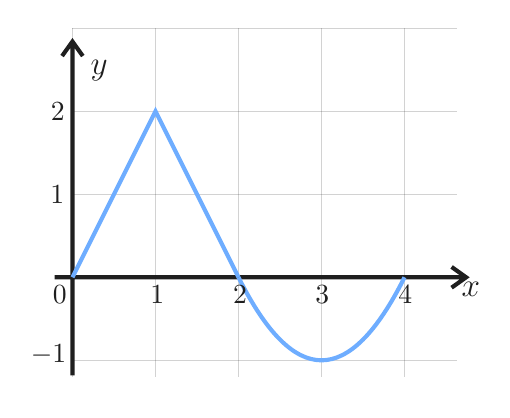
\begin{tikzpicture}[x=0.75pt,y=0.75pt,yscale=-1,xscale=1]
%uncomment if require: \path (0,168); %set diagram left start at 0, and has height of 168

%Shape: Grid [id:dp3870395650733016] 
\draw  [draw opacity=0] (23.7,-4.4) -- (208.89,-4.4) -- (208.89,163.74) -- (23.7,163.74) -- cycle ; \draw  [color={rgb, 255:red, 31; green, 31; blue, 31 }  ,draw opacity=0.2 ] (23.7,-4.4) -- (23.7,163.74)(63.7,-4.4) -- (63.7,163.74)(103.7,-4.4) -- (103.7,163.74)(143.7,-4.4) -- (143.7,163.74)(183.7,-4.4) -- (183.7,163.74) ; \draw  [color={rgb, 255:red, 31; green, 31; blue, 31 }  ,draw opacity=0.2 ] (23.7,-4.4) -- (208.89,-4.4)(23.7,35.6) -- (208.89,35.6)(23.7,75.6) -- (208.89,75.6)(23.7,115.6) -- (208.89,115.6)(23.7,155.6) -- (208.89,155.6) ; \draw  [color={rgb, 255:red, 31; green, 31; blue, 31 }  ,draw opacity=0.2 ]  ;
%Shape: Axis 2D [id:dp1245822243275887] 
\draw [color={rgb, 255:red, 31; green, 31; blue, 31 }  ,draw opacity=1 ][line width=1.5]  (15.11,115.6) -- (213.38,115.6)(23.7,2) -- (23.7,162.8) (206.38,110.6) -- (213.38,115.6) -- (206.38,120.6) (18.7,9) -- (23.7,2) -- (28.7,9)  ;
%Straight Lines [id:da8527565778929875] 
\draw [color={rgb, 255:red, 110; green, 173; blue, 255 }  ,draw opacity=1 ][line width=1.5]    (23.7,115.6) -- (63.7,35.6) -- (103.7,115.6) ;
%Shape: Parabola [id:dp3769236686385484] 
\draw  [color={rgb, 255:red, 110; green, 173; blue, 255 }  ,draw opacity=1 ][line width=1.5]  (103.7,115.6) .. controls (130.37,168.93) and (157.03,168.93) .. (183.7,115.6) ;

% Text Node
\draw (31.2,9.5) node [anchor=north west][inner sep=0.75pt]  [font=\large,color={rgb, 255:red, 31; green, 31; blue, 31 }  ,opacity=1 ]  {$y$};
% Text Node
\draw (210,116.9) node [anchor=north west][inner sep=0.75pt]  [font=\large,color={rgb, 255:red, 31; green, 31; blue, 31 }  ,opacity=1 ]  {$x$};
% Text Node
\draw (13,118.2) node [anchor=north west][inner sep=0.75pt]  [color={rgb, 255:red, 31; green, 31; blue, 31 }  ,opacity=1 ]  {$0$};
% Text Node
\draw (60,118.3) node [anchor=north west][inner sep=0.75pt]  [color={rgb, 255:red, 31; green, 31; blue, 31 }  ,opacity=1 ]  {$1$};
% Text Node
\draw (99.9,118.6) node [anchor=north west][inner sep=0.75pt]  [color={rgb, 255:red, 31; green, 31; blue, 31 }  ,opacity=1 ]  {$2$};
% Text Node
\draw (139.5,118.2) node [anchor=north west][inner sep=0.75pt]  [color={rgb, 255:red, 31; green, 31; blue, 31 }  ,opacity=1 ]  {$3$};
% Text Node
\draw (179.5,118.2) node [anchor=north west][inner sep=0.75pt]  [color={rgb, 255:red, 31; green, 31; blue, 31 }  ,opacity=1 ]  {$4$};
% Text Node
\draw (12,30.2) node [anchor=north west][inner sep=0.75pt]  [color={rgb, 255:red, 31; green, 31; blue, 31 }  ,opacity=1 ]  {$2$};
% Text Node
\draw (11.8,70.2) node [anchor=north west][inner sep=0.75pt]  [color={rgb, 255:red, 31; green, 31; blue, 31 }  ,opacity=1 ]  {$1$};
% Text Node
\draw (2.4,147) node [anchor=north west][inner sep=0.75pt]  [color={rgb, 255:red, 31; green, 31; blue, 31 }  ,opacity=1 ]  {$-1$};


\end{tikzpicture}
    \par}

maka
\begin{enumerate}
    \item $g^\prime(x) < 0$ pada selang $(a, b)$ dengan $a = \fillin$ dan $b = \fillin$
    \item Titik stasioner dari fungsi $g$ adalah $x = \fillin$
\end{enumerate}
\begin{proof}
    Catat bahwa turunan dari suatu fungsi menyatakan gradien garis singgung pada grafik fungsi tersebut. Beberapa garis singgung pada grafik fungsi $g$ digambarkan oleh garis merah pada ilustrasi berikut.

    {\centering
    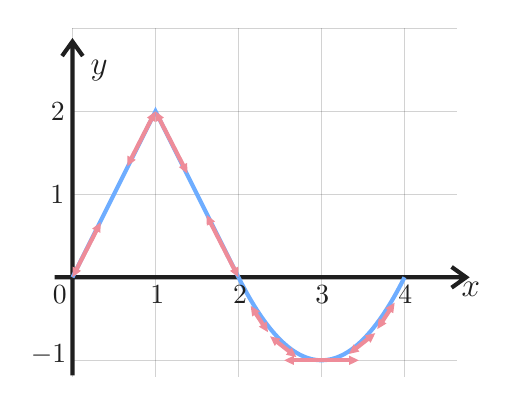
\begin{tikzpicture}[x=0.75pt,y=0.75pt,yscale=-1,xscale=1]
%uncomment if require: \path (0,168); %set diagram left start at 0, and has height of 168

%Shape: Grid [id:dp3870395650733016] 
\draw  [draw opacity=0] (23.7,-4.4) -- (208.89,-4.4) -- (208.89,163.74) -- (23.7,163.74) -- cycle ; \draw  [color={rgb, 255:red, 31; green, 31; blue, 31 }  ,draw opacity=0.2 ] (23.7,-4.4) -- (23.7,163.74)(63.7,-4.4) -- (63.7,163.74)(103.7,-4.4) -- (103.7,163.74)(143.7,-4.4) -- (143.7,163.74)(183.7,-4.4) -- (183.7,163.74) ; \draw  [color={rgb, 255:red, 31; green, 31; blue, 31 }  ,draw opacity=0.2 ] (23.7,-4.4) -- (208.89,-4.4)(23.7,35.6) -- (208.89,35.6)(23.7,75.6) -- (208.89,75.6)(23.7,115.6) -- (208.89,115.6)(23.7,155.6) -- (208.89,155.6) ; \draw  [color={rgb, 255:red, 31; green, 31; blue, 31 }  ,draw opacity=0.2 ]  ;
%Shape: Axis 2D [id:dp1245822243275887] 
\draw [color={rgb, 255:red, 31; green, 31; blue, 31 }  ,draw opacity=1 ][line width=1.5]  (15.11,115.6) -- (213.38,115.6)(23.7,2) -- (23.7,162.8) (206.38,110.6) -- (213.38,115.6) -- (206.38,120.6) (18.7,9) -- (23.7,2) -- (28.7,9)  ;
%Straight Lines [id:da8527565778929875] 
\draw [color={rgb, 255:red, 110; green, 173; blue, 255 }  ,draw opacity=1 ][line width=1.5]    (23.7,115.6) -- (63.7,35.6) -- (103.7,115.6) ;
%Shape: Parabola [id:dp3769236686385484] 
\draw  [color={rgb, 255:red, 110; green, 173; blue, 255 }  ,draw opacity=1 ][line width=1.5]  (103.7,115.6) .. controls (130.37,168.93) and (157.03,168.93) .. (183.7,115.6) ;
%Straight Lines [id:da04042907965545739] 
\draw [color={rgb, 255:red, 238; green, 140; blue, 153 }  ,draw opacity=1 ][line width=1.5]    (111.8,132.72) -- (115.73,138.7) ;
\draw [shift={(117.93,142.04)}, rotate = 236.66] [fill={rgb, 255:red, 238; green, 140; blue, 153 }  ,fill opacity=1 ][line width=0.08]  [draw opacity=0] (4.64,-2.23) -- (0,0) -- (4.64,2.23) -- cycle    ;
\draw [shift={(109.6,129.38)}, rotate = 56.66] [fill={rgb, 255:red, 238; green, 140; blue, 153 }  ,fill opacity=1 ][line width=0.08]  [draw opacity=0] (4.64,-2.23) -- (0,0) -- (4.64,2.23) -- cycle    ;
%Straight Lines [id:da4797917404336065] 
\draw [color={rgb, 255:red, 238; green, 140; blue, 153 }  ,draw opacity=1 ][line width=1.5]    (90.13,89.13) -- (101.87,112.04) ;
\draw [shift={(103.7,115.6)}, rotate = 242.85] [fill={rgb, 255:red, 238; green, 140; blue, 153 }  ,fill opacity=1 ][line width=0.08]  [draw opacity=0] (4.64,-2.23) -- (0,0) -- (4.64,2.23) -- cycle    ;
\draw [shift={(88.3,85.57)}, rotate = 62.85] [fill={rgb, 255:red, 238; green, 140; blue, 153 }  ,fill opacity=1 ][line width=0.08]  [draw opacity=0] (4.64,-2.23) -- (0,0) -- (4.64,2.23) -- cycle    ;
%Straight Lines [id:da3366888937622974] 
\draw [color={rgb, 255:red, 238; green, 140; blue, 153 }  ,draw opacity=1 ][line width=1.5]    (25.52,112.04) -- (33.73,96.04) -- (35.47,92.63) ;
\draw [shift={(37.3,89.07)}, rotate = 117.15] [fill={rgb, 255:red, 238; green, 140; blue, 153 }  ,fill opacity=1 ][line width=0.08]  [draw opacity=0] (4.64,-2.23) -- (0,0) -- (4.64,2.23) -- cycle    ;
\draw [shift={(23.7,115.6)}, rotate = 297.15] [fill={rgb, 255:red, 238; green, 140; blue, 153 }  ,fill opacity=1 ][line width=0.08]  [draw opacity=0] (4.64,-2.23) -- (0,0) -- (4.64,2.23) -- cycle    ;
%Straight Lines [id:da7531192535470417] 
\draw [color={rgb, 255:red, 238; green, 140; blue, 153 }  ,draw opacity=1 ][line width=1.5]    (65.53,39.16) -- (77.27,62.07) ;
\draw [shift={(79.1,65.62)}, rotate = 242.85] [fill={rgb, 255:red, 238; green, 140; blue, 153 }  ,fill opacity=1 ][line width=0.08]  [draw opacity=0] (4.64,-2.23) -- (0,0) -- (4.64,2.23) -- cycle    ;
\draw [shift={(63.7,35.6)}, rotate = 62.85] [fill={rgb, 255:red, 238; green, 140; blue, 153 }  ,fill opacity=1 ][line width=0.08]  [draw opacity=0] (4.64,-2.23) -- (0,0) -- (4.64,2.23) -- cycle    ;
%Straight Lines [id:da5619695433273342] 
\draw [color={rgb, 255:red, 238; green, 140; blue, 153 }  ,draw opacity=1 ][line width=1.5]    (51.92,58.57) -- (60.13,42.56) -- (61.88,39.16) ;
\draw [shift={(63.7,35.6)}, rotate = 117.15] [fill={rgb, 255:red, 238; green, 140; blue, 153 }  ,fill opacity=1 ][line width=0.08]  [draw opacity=0] (4.64,-2.23) -- (0,0) -- (4.64,2.23) -- cycle    ;
\draw [shift={(50.1,62.12)}, rotate = 297.15] [fill={rgb, 255:red, 238; green, 140; blue, 153 }  ,fill opacity=1 ][line width=0.08]  [draw opacity=0] (4.64,-2.23) -- (0,0) -- (4.64,2.23) -- cycle    ;
%Straight Lines [id:da1149150142922577] 
\draw [color={rgb, 255:red, 238; green, 140; blue, 153 }  ,draw opacity=1 ][line width=1.5]    (122.07,146.52) -- (128.46,151.56) ;
\draw [shift={(131.6,154.04)}, rotate = 218.29] [fill={rgb, 255:red, 238; green, 140; blue, 153 }  ,fill opacity=1 ][line width=0.08]  [draw opacity=0] (4.64,-2.23) -- (0,0) -- (4.64,2.23) -- cycle    ;
\draw [shift={(118.93,144.04)}, rotate = 38.29] [fill={rgb, 255:red, 238; green, 140; blue, 153 }  ,fill opacity=1 ][line width=0.08]  [draw opacity=0] (4.64,-2.23) -- (0,0) -- (4.64,2.23) -- cycle    ;
%Straight Lines [id:da8083183763044457] 
\draw [color={rgb, 255:red, 238; green, 140; blue, 153 }  ,draw opacity=1 ][line width=1.5]    (129.7,155.6) -- (157.7,155.6) ;
\draw [shift={(161.7,155.6)}, rotate = 180] [fill={rgb, 255:red, 238; green, 140; blue, 153 }  ,fill opacity=1 ][line width=0.08]  [draw opacity=0] (4.64,-2.23) -- (0,0) -- (4.64,2.23) -- cycle    ;
\draw [shift={(125.7,155.6)}, rotate = 0] [fill={rgb, 255:red, 238; green, 140; blue, 153 }  ,fill opacity=1 ][line width=0.08]  [draw opacity=0] (4.64,-2.23) -- (0,0) -- (4.64,2.23) -- cycle    ;
%Straight Lines [id:da0354177747691129] 
\draw [color={rgb, 255:red, 238; green, 140; blue, 153 }  ,draw opacity=1 ][line width=1.5]    (176.73,131.19) -- (172.8,137.17) ;
\draw [shift={(170.6,140.51)}, rotate = 303.34] [fill={rgb, 255:red, 238; green, 140; blue, 153 }  ,fill opacity=1 ][line width=0.08]  [draw opacity=0] (4.64,-2.23) -- (0,0) -- (4.64,2.23) -- cycle    ;
\draw [shift={(178.93,127.84)}, rotate = 123.34] [fill={rgb, 255:red, 238; green, 140; blue, 153 }  ,fill opacity=1 ][line width=0.08]  [draw opacity=0] (4.64,-2.23) -- (0,0) -- (4.64,2.23) -- cycle    ;
%Straight Lines [id:da7111405748526216] 
\draw [color={rgb, 255:red, 238; green, 140; blue, 153 }  ,draw opacity=1 ][line width=1.5]    (166.46,144.99) -- (160.07,150.03) ;
\draw [shift={(156.93,152.51)}, rotate = 321.71] [fill={rgb, 255:red, 238; green, 140; blue, 153 }  ,fill opacity=1 ][line width=0.08]  [draw opacity=0] (4.64,-2.23) -- (0,0) -- (4.64,2.23) -- cycle    ;
\draw [shift={(169.6,142.51)}, rotate = 141.71] [fill={rgb, 255:red, 238; green, 140; blue, 153 }  ,fill opacity=1 ][line width=0.08]  [draw opacity=0] (4.64,-2.23) -- (0,0) -- (4.64,2.23) -- cycle    ;

% Text Node
\draw (31.2,9.5) node [anchor=north west][inner sep=0.75pt]  [font=\large,color={rgb, 255:red, 31; green, 31; blue, 31 }  ,opacity=1 ]  {$y$};
% Text Node
\draw (210,116.9) node [anchor=north west][inner sep=0.75pt]  [font=\large,color={rgb, 255:red, 31; green, 31; blue, 31 }  ,opacity=1 ]  {$x$};
% Text Node
\draw (13,118.2) node [anchor=north west][inner sep=0.75pt]  [color={rgb, 255:red, 31; green, 31; blue, 31 }  ,opacity=1 ]  {$0$};
% Text Node
\draw (60,118.3) node [anchor=north west][inner sep=0.75pt]  [color={rgb, 255:red, 31; green, 31; blue, 31 }  ,opacity=1 ]  {$1$};
% Text Node
\draw (99.9,118.6) node [anchor=north west][inner sep=0.75pt]  [color={rgb, 255:red, 31; green, 31; blue, 31 }  ,opacity=1 ]  {$2$};
% Text Node
\draw (139.5,118.2) node [anchor=north west][inner sep=0.75pt]  [color={rgb, 255:red, 31; green, 31; blue, 31 }  ,opacity=1 ]  {$3$};
% Text Node
\draw (179.5,118.2) node [anchor=north west][inner sep=0.75pt]  [color={rgb, 255:red, 31; green, 31; blue, 31 }  ,opacity=1 ]  {$4$};
% Text Node
\draw (12,30.2) node [anchor=north west][inner sep=0.75pt]  [color={rgb, 255:red, 31; green, 31; blue, 31 }  ,opacity=1 ]  {$2$};
% Text Node
\draw (11.8,70.2) node [anchor=north west][inner sep=0.75pt]  [color={rgb, 255:red, 31; green, 31; blue, 31 }  ,opacity=1 ]  {$1$};
% Text Node
\draw (2.4,147) node [anchor=north west][inner sep=0.75pt]  [color={rgb, 255:red, 31; green, 31; blue, 31 }  ,opacity=1 ]  {$-1$};


\end{tikzpicture}
    \par}

    \begin{enumerate}[label=(\alph*)]
        \item $g^\prime(x) < 0$ ketika $g(x)$ monoton turun, yakni ketika gradien garis singgung bernilai negatif. Secara grafis, pada kondisi ini gradien garis singgungnya menurun. Kondisi tersebut tercapai pada selang $(1,3)$. Jadi, $a = 1$ dan $b = 3$. \qed
        \item Titik stasioner tercapai ketika $g^\prime(x) = 0$, yakni garis singgung grafik mendatar. Kondisi tersebut tercapai ketika $x = 3$. Titik $x = 1$ tidak termasuk titik stasioner karena turunan dari sisi kiri dan sisi kanannya berbeda, yang secara grafis menghasilkan titik yang lancip. \qed
    \end{enumerate}
\end{proof}\vspace{1em}
\end{enumerate}


\pagebreak
\section*{Bagian B}
\begin{enumerate}
    \item Hitunglah $\displaystyle \lim_{x \to 2} \frac{x^2 - x - 2}{x^2 - 4}$.
    
    \begin{proof}
        Mensubstitusikan $x = 2$ akan memberikan bentuk tak tentu $0/0$ sehingga kita perlu sederhanakan dahulu.
        
        \vspace{-2em}
        \begin{align*}
            \lim_{x \to 2} \frac{x^2 - x - 2}{x^2 - 4}  &= \lim_{x \to 2} \frac{\cancel{(x - 2)}(x + 1)}{\cancel{(x - 2)}(x + 2)} \\[.5em]
                                                        &= \lim_{x \to 2} \frac{x + 1}{x + 2}   \\[.5em]
                                                        &= \frac{2 + 1}{2 + 2}                  \\[.5em]
                                                        &= \frac{3}{4} \qed
        \end{align*}
    \end{proof}\vspace{1em}
    
    \item Jika $f(x) = \sqrt{x^2 + 5}$, hitunglah $f^\prime(2)$.
    
    \begin{proof}
        Untuk menurunkan $f(x)$ kita perlu menerapkan aturan rantai.
        \par Misalkan $u = x^2 + 5$ sehingga $$ \dv{u}{x} = 2x.$$ 
        \par Di samping itu, $f(x) = \sqrt{u} = u^{1/2}$ sehingga $$ \dv{f(x)}{u} = \frac{1}{2}u^{-1/2} = \frac{1}{2\sqrt{u}}.$$
        \par Akibatnya, dengan aturan rantai kita peroleh

        \vspace{-1em}
        \begin{align*}
            f^\prime(x) = \dv{f(x)}{x}  &= \dv{f(x)}{u} \cdot \dv{u}{x} \\[.5em]
                                        &= \frac{1}{\cancel{2}\sqrt{u}} \cdot \cancel{2}x \\[.5em]
                                        &= \frac{x}{\sqrt{u}}           \\[.5em]
                                        &= \frac{x}{\sqrt{x^2 + 5}}            \\[.5em]
                            f^\prime(2) &= \frac{2}{\sqrt{2^2 + 5}}            \\[.5em]
                                        &= \frac{2}{3} \qed
        \end{align*}
    \end{proof}\vspace{1em}

    
    \item Tentukan nilai minimum dan maksimum dari fungsi $f(x) = x + \dfrac{4}{x}$ pada selang $[1,5]$.

    \begin{proof}
        Pertama, kita cari titik-titik kritis dari fungsi tersebut.
        \textit{Titik Ujung Selang}\\
        Titik ujung selangnya adalah $x = 1$ dan $x = 5$.
        \textit{Titik Stasioner}\\
        Turunan pertama $f(x) = x + 4x^{-1}$ adalah
        \[f^\prime(x) = 1 - 4x^{-2} = 1 - \frac{4}{x^2} = \frac{x^2 - 4}{x^2} = \frac{(x-2)(x+2)}{x^2}.\]

        Pembuat nol $f^\prime(x)$ adalah
            \[\frac{(x-2)(x+2)}{x^2} = 0 \iff x = -2 \lor x = 2 \]

        Mengingat $x = -2$ berada di luar selang $[1,5]$, titik stasioner pada selang ini adalah $x = 2$.
        \textit{Titik Singular}\\
        Titik singular terjadi ketika $f^\prime(x)$ tak terdefinisi, yakni ketika penyebutnya nol, yang terjadi pada $x = 0$. Akan tetapi, $f(x)$ juga tidak terdefinisi pada $x = 0$ sehingga kita tidak perlu pertimbangakan titik ini.

        Selanjutnya, hitung nilai $f$ untuk titik-titik kritis yang sudah didapatkan:
        \begin{align*}
            f(1)    &= 1 + \frac{4}{1}      = 5             \\
            f(2)    &= 2 + \frac{4}{2}      = 4             \\
            f(5)    &= 5 + \frac{4}{5}      = \frac{29}{5}
        \end{align*}

        Dengan membandingkan seluruh nilai $f$ di atas, didapatkan nilai minimum $f(2) = 4$ dan nilai maksimum $f(5) = \dfrac{29}{5}$. \qed
        
    \end{proof}\vspace{1em}

    Nilai minimum tercapai di $x = a$ jika $f^\prime(x) < 0$ (monoton turun) di kiri $a$ lalu $f^\prime(x) > 0$ (monoton naik) di kanannya, dan sebaliknya berlaku untuk nilai maksimum. Jadi,

    
    \item Suatu daerah $D$ di kuadran I dibatasi oleh kurva $y = \sqrt{2x}$, garis $x = 3$, dan sumbu-$x$.
    
    {\centering
\tikzset{every picture/.style={line width=0.75pt}} %set default line width to 0.75pt        
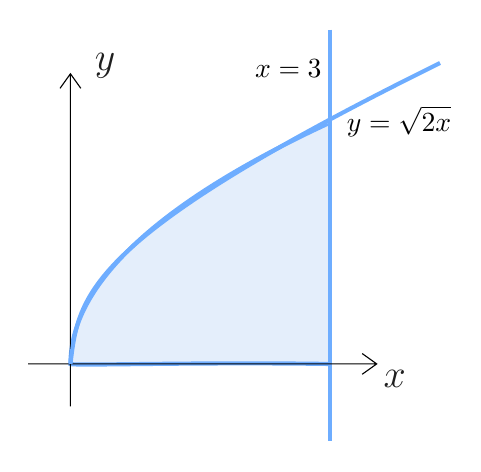
\begin{tikzpicture}[x=0.75pt,y=0.75pt,yscale=-1,xscale=1]
%uncomment if require: \path (0,179); %set diagram left start at 0, and has height of 179

%Curve Lines [id:da14093263278979817] 
\draw [color={rgb, 255:red, 110; green, 173; blue, 255 }  ,draw opacity=1 ][fill={rgb, 255:red, 164; green, 198; blue, 243 }  ,fill opacity=0.3 ][line width=1.5]    (170.4,157.98) .. controls (105.47,156.99) and (47.4,158.98) .. (46.33,157.96) .. controls (46.4,130.98) and (67.4,89.98) .. (170.33,42.22) ;
%Straight Lines [id:da007777140770855118] 
\draw [color={rgb, 255:red, 110; green, 173; blue, 255 }  ,draw opacity=1 ][line width=1.5]    (171.33,-3.04) -- (171.33,195.28) ;
%Shape: Axis 2D [id:dp08198994155095618] 
\draw  (26,157.96) -- (193.89,157.96)(46.33,18.18) -- (46.33,178.4) (186.89,152.96) -- (193.89,157.96) -- (186.89,162.96) (41.33,25.18) -- (46.33,18.18) -- (51.33,25.18)  ;
%Curve Lines [id:da09352803496149553] 
\draw [color={rgb, 255:red, 110; green, 173; blue, 255 }  ,draw opacity=1 ][line width=1.5]    (46.33,157.96) .. controls (50.4,124.98) and (52.4,97.98) .. (224.4,12.98) ;

% Text Node
\draw (56.84,7.28) node [anchor=north west][inner sep=0.75pt]  [font=\Large,color={rgb, 255:red, 31; green, 31; blue, 31 }  ,opacity=1 ]  {$y$};
% Text Node
\draw (196,160) node [anchor=north west][inner sep=0.75pt]  [font=\Large,color={rgb, 255:red, 31; green, 31; blue, 31 }  ,opacity=1 ]  {$x$};
% Text Node
\draw (134,10) node [anchor=north west][inner sep=0.75pt]    {$x=3$};
% Text Node
\draw (178.31,32.4) node [anchor=north west][inner sep=0.75pt]    {$y=\sqrt{2x}$};


\end{tikzpicture}
\par}
    
    Tentukan volume benda pejal yang diperoleh dengan memutar daerah $D$ mengelilingi sumbu-$x$.

    \begin{proof}
        Perhatikan skema berikut.

        {\centering
        

\tikzset{every picture/.style={line width=0.75pt}} %set default line width to 0.75pt        

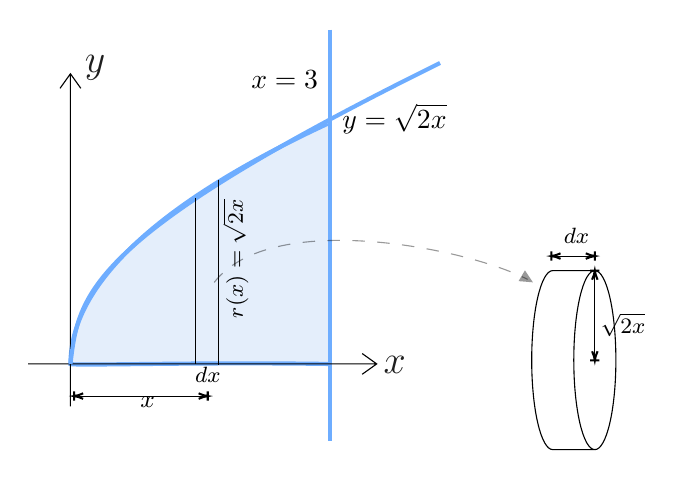
\begin{tikzpicture}[x=0.75pt,y=0.75pt,yscale=-1,xscale=1]
%uncomment if require: \path (0,208); %set diagram left start at 0, and has height of 208

%Curve Lines [id:da17823650509833455] 
\draw [color={rgb, 255:red, 110; green, 173; blue, 255 }  ,draw opacity=1 ][fill={rgb, 255:red, 164; green, 198; blue, 243 }  ,fill opacity=0.3 ][line width=1.5]    (170.4,157.98) .. controls (105.47,156.99) and (47.4,158.98) .. (46.33,157.96) .. controls (46.4,130.98) and (67.4,89.98) .. (170.33,42.22) ;
%Straight Lines [id:da3182604894630108] 
\draw [color={rgb, 255:red, 110; green, 173; blue, 255 }  ,draw opacity=1 ][line width=1.5]    (171.33,-3.04) -- (171.33,195.28) ;
%Shape: Axis 2D [id:dp31880702696074437] 
\draw  (26,157.96) -- (193.89,157.96)(46.33,18.18) -- (46.33,178.4) (186.89,152.96) -- (193.89,157.96) -- (186.89,162.96) (41.33,25.18) -- (46.33,18.18) -- (51.33,25.18)  ;
%Curve Lines [id:da3176601313589229] 
\draw [color={rgb, 255:red, 110; green, 173; blue, 255 }  ,draw opacity=1 ][line width=1.5]    (46.33,157.96) .. controls (50.4,124.98) and (52.4,97.98) .. (224.4,12.98) ;
%Straight Lines [id:da5585343567206977] 
\draw    (106.8,77.86) -- (106.8,157.86) ;
%Straight Lines [id:da9297714961840782] 
\draw    (117.48,69.46) -- (117.48,158.46) ;
%Straight Lines [id:da6001018318976798] 
\draw    (112.48,173.46) -- (48.08,173.46) ;
\draw [shift={(48.08,173.46)}, rotate = 360] [color={rgb, 255:red, 0; green, 0; blue, 0 }  ][line width=0.75]    (0,2.24) -- (0,-2.24)(4.37,-1.32) .. controls (2.78,-0.56) and (1.32,-0.12) .. (0,0) .. controls (1.32,0.12) and (2.78,0.56) .. (4.37,1.32)   ;
\draw [shift={(112.48,173.46)}, rotate = 180] [color={rgb, 255:red, 0; green, 0; blue, 0 }  ][line width=0.75]    (0,2.24) -- (0,-2.24)(4.37,-1.32) .. controls (2.78,-0.56) and (1.32,-0.12) .. (0,0) .. controls (1.32,0.12) and (2.78,0.56) .. (4.37,1.32)   ;
%Shape: Can [id:dp6751386518745286] 
\draw   (298.99,199.26) -- (278.71,199.26) .. controls (273.11,199.26) and (268.57,179.95) .. (268.57,156.13) .. controls (268.57,132.31) and (273.11,113) .. (278.71,113) -- (298.99,113) .. controls (304.59,113) and (309.13,132.31) .. (309.13,156.13) .. controls (309.13,179.95) and (304.59,199.26) .. (298.99,199.26) .. controls (293.39,199.26) and (288.85,179.95) .. (288.85,156.13) .. controls (288.85,132.31) and (293.39,113) .. (298.99,113) ;
%Straight Lines [id:da9322855707635862] 
\draw    (298.99,113) -- (298.99,156.26) ;
\draw [shift={(298.99,156.26)}, rotate = 270] [color={rgb, 255:red, 0; green, 0; blue, 0 }  ][line width=0.75]    (0,2.24) -- (0,-2.24)(4.37,-1.32) .. controls (2.78,-0.56) and (1.32,-0.12) .. (0,0) .. controls (1.32,0.12) and (2.78,0.56) .. (4.37,1.32)   ;
\draw [shift={(298.99,113)}, rotate = 90] [color={rgb, 255:red, 0; green, 0; blue, 0 }  ][line width=0.75]    (0,2.24) -- (0,-2.24)(4.37,-1.32) .. controls (2.78,-0.56) and (1.32,-0.12) .. (0,0) .. controls (1.32,0.12) and (2.78,0.56) .. (4.37,1.32)   ;
%Straight Lines [id:da16415778473892462] 
\draw    (298.99,106) -- (278.09,106) ;
\draw [shift={(278.09,106)}, rotate = 360] [color={rgb, 255:red, 0; green, 0; blue, 0 }  ][line width=0.75]    (0,2.24) -- (0,-2.24)(4.37,-1.32) .. controls (2.78,-0.56) and (1.32,-0.12) .. (0,0) .. controls (1.32,0.12) and (2.78,0.56) .. (4.37,1.32)   ;
\draw [shift={(298.99,106)}, rotate = 180] [color={rgb, 255:red, 0; green, 0; blue, 0 }  ][line width=0.75]    (0,2.24) -- (0,-2.24)(4.37,-1.32) .. controls (2.78,-0.56) and (1.32,-0.12) .. (0,0) .. controls (1.32,0.12) and (2.78,0.56) .. (4.37,1.32)   ;
%Curve Lines [id:da4934197227065591] 
\draw [color={rgb, 255:red, 0; green, 0; blue, 0 }  ,draw opacity=0.4 ] [dash pattern={on 4.5pt off 4.5pt}]  (115.6,118.7) .. controls (142.72,83.35) and (236.87,101.86) .. (266.59,117.24) ;
\draw [shift={(269.16,118.66)}, rotate = 210.58] [fill={rgb, 255:red, 0; green, 0; blue, 0 }  ,fill opacity=0.4 ][line width=0.08]  [draw opacity=0] (6.25,-3) -- (0,0) -- (6.25,3) -- cycle    ;

% Text Node
\draw (52.04,8.08) node [anchor=north west][inner sep=0.75pt]  [font=\Large,color={rgb, 255:red, 31; green, 31; blue, 31 }  ,opacity=1 ]  {$y$};
% Text Node
\draw (195.94,152.95) node [anchor=north west][inner sep=0.75pt]  [font=\Large,color={rgb, 255:red, 31; green, 31; blue, 31 }  ,opacity=1 ]  {$x$};
% Text Node
\draw (118.4,137.2) node [anchor=north west][inner sep=0.75pt]  [font=\footnotesize,rotate=-270]  {$r( x) =\sqrt{2x}$};
% Text Node
\draw (105.2,158.2) node [anchor=north west][inner sep=0.75pt]  [font=\footnotesize]  {$dx$};
% Text Node
\draw (132.2,15.2) node [anchor=north west][inner sep=0.75pt]    {$x=3$};
% Text Node
\draw (176.11,31.2) node [anchor=north west][inner sep=0.75pt]    {$y=\sqrt{2x}$};
% Text Node
\draw (78.8,172.3) node [anchor=north west][inner sep=0.75pt]  [font=\small]  {$x$};
% Text Node
\draw (282.8,91.28) node [anchor=north west][inner sep=0.75pt]  [font=\footnotesize]  {$dx$};
% Text Node
\draw (300.6,132.28) node [anchor=north west][inner sep=0.75pt]  [font=\footnotesize]  {$\sqrt{2x}$};


\end{tikzpicture}
        \par}
        
        Taksiran volume satu irisan pada daerah $D$ adalah 
        \[\dd{V} = \pi \qty(\sqrt{2x})^2 \dd{x} = 2 \pi x \dd{x}.\]

        Daerah $D$ memanjang dari $x = 0$ hingga $x = 3$ sehingga volumenya adalah

        \begin{align*}
            V   &= \int_{0}^{3} \dd{V}                                  \\[.5em]
                &= \int_{0}^{3} 2 \pi x \dd{x}                          \\[.5em]
                &= \cancel{2}\pi \frac{x^2}{\cancel{2}} \Big|_{0}^{3}   \\[.5em]
                &= \pi{x^2} \Big|_{0}^{3}                               \\[.5em]
                &= \pi(3^2 - 0^2)                                       \\[.5em]
                &= 9\pi
        \end{align*}

        %\textit{Metode Kulit Tabung}. Perhatikan skema berikut.

        %Taksiran volume satu irisan pada daerah $D$ adalah 
        %\[\dd{V} = 2\pi \qty(3 - \frac{y^2}{2}) \dd{y}\]
%
        %sehingga volume daerah $D$ adalah
%
        %\begin{align*}
        %    V   &= \int_{0}^{\sqrt{6}} \dd{V}                               \\[.5em]
        %        &= \int_{0}^{\sqrt{6}} 2\pi \qty(3 - \frac{y^2}{2}) \dd{y}  \\[.5em]
        %        &= 2\pi (3 - \frac{y^3}{6}) \Big|_{0}^{\sqrt{6}}
        %\end{align*}
    
    \end{proof}\vspace{1em}
    
    \item Tentukan solusi umum persamaan diferensial $\displaystyle \dv{y}{t} = 3t^2y$ dengan $y(t) > 0$.
    \begin{proof}
        Persamaan diferensial ini adalah persmaaan diferensial separabel di mana kita bisa sepenuhnya memisahkan variabel $y$ dan $t$ pada ruas yang berbeda:

        \vspace{-1.5em}
        \begin{align*}
            \dv{y}{t}           &= 3t^2y        \\[.5em]
            \frac{1}{y}\dd{y}   &= 3t^2 \dd{t}
        \end{align*}
        
        Dengan mengintegralkan kedua ruas, diperoleh

        \vspace{-1.5em}
        \begin{align*}
            \int \frac{1}{y} \dd{y} &= \int 3t^2 \dd{t} \\[.5em]
            \ln|y|                  &= t^3 + C
        \end{align*}

        Pangkatkan kedua ruas terhadap $e$ sehingga

        \vspace{-1.5em}
        \begin{align*}
            e^{\ln |y|} &= e^{t^3 + C} \\[.5em]
            |y|         &= e^{t^3 + C}
        \end{align*}
        
        Catat bahwa $|y| = y$ mengingat $y > 0$. Dengan demikian, solusi umum persamaan diferensial tersebut adalah
        \[ y = e^{t^3 + C} \qed\]
    \end{proof}\vspace{1em}
\end{enumerate}

\vspace{5em}

\garis{Kite}{Kite}
Arsip soal oleh @PanduGus di Twitter\\
Solusi dan \textit{typesetting} di LaTeX oleh Z. Nayaka Athadiansyah
\garis{Kite}{Kite}

\end{document}